
\subsection{Multi-Label Object Classification}
% Describe here the CNN architecture.

We have designed our model with classic 2D Convolutional neural network.
Our network architecture is represented in fig:cnn.
The network model is designed for multiclass classification of point cloud object. Convolutional Neural network gives promising result of object model with spatial data. CNN effectively learns the feature recognition of planes, corners, and the edge of the object model. Our Network model is designed with 4 Convolutional layers, where each layer filter is expected to recognize
planes, corners, edges, and distribution of the objects per orientation.
other layers learn the global label for the input grid from the knowledge passed by each layer.

Input layer:
The network model takes a fixed-size grid of NxM voxels as an input.we have used N=70 and M=100 for our model requirements.
Each voxel grid contains the consolidated lidar point-clouds point into the voxels. Each voxel is of size k, we have used k=0.1
which generates the input voxel grids. The input layer forwards each object input to the 1st layer of Convolutional.


Convolutional Layer(input,f,s):
There is 4 Convolutional layer in our architecture to learn features on each orientation.
The first convolutional layer feed on three-dimensional input of size NxMxf from the input layer, a filter size=f and number of filter to be applied.
The filter-size provided to convolutional layer is 5x5 with 16 such filters to be applied on the input.
The convolutional layer equates filter f by apply convolutional on input dimension to create a feature map as output.
The Convolutional layer learns about the spatial planes, edges, and distribution in the object, the convolutional layer passes the output to the rectified nonlinearity unit(Relu) before feeding it forward to next Layers.

Max Pooling layer:
The pooling layer is added to downsample the by a factor of vector d, in our network model d = [1,2,2,1].
the max pooling layer is after each alternative convolutional layer, it downsamples the dimension of the feature map with their maximums.

Dropout Layer:
Dropout layer is used for reducing overfitting. As the network is executed on the iterative model with a feed forward network.
The Model network tends to overfit on the data. Dropout layer drops random samples from the feature map.

Fully Connected Layer.
As fully connected layers contain n output neurons.
each neuron of the output is a learned linear combination of all the outputs from the previous layer,
passed through a nonlinearity.
We use ReLUs to save the final output layer, where the number of outputs corresponds
to the number of class labels and a softmax nonlinearity is used to provide a probabilistic output.


Our Network model starts with an input layer feeding to convolution layer with ReLu then
another Conv layer with ReLu and max pool layer then passing input to another batch of Conv layers
with Relu and Conv layer with Relu and max pool, then the feature map is flattened to be feed-forwarded to
fully connected layer with ReLu, then random samples are dropped with dropout layers
and finally fed to a fully connected layer and softmax to classify the object into multiclass.

\begin{figure*}[!h]
     \begin{center}
       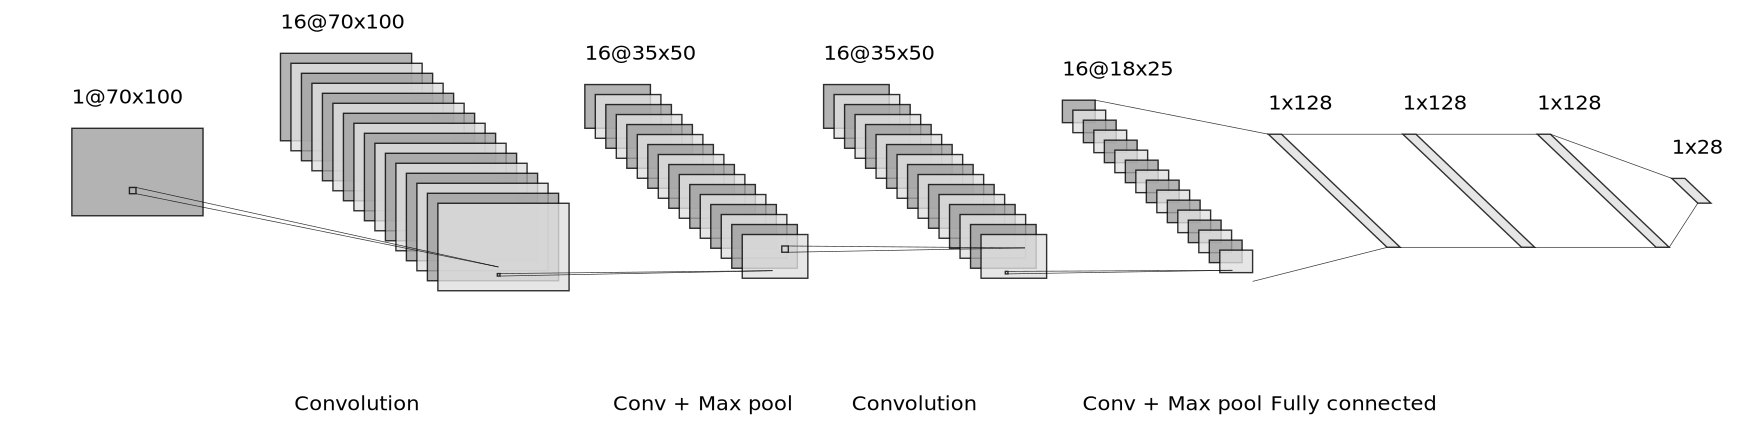
\includegraphics[width=1.1\textwidth]{./images/object_net.pdf}
       \caption{Overview of Convolutional Neural Network Layers}
       \label{fig:cnn}
     \end{center}
\end{figure*}

\subsection{3D CNN experiment}
We experimented with 3D CNN as dataset could be transformed into the
input of 3D CNN being a 3D point cloud dataset. Our approach was to convert point clouds into a set of voxels by voxelization. Voxelization is the process of conversion of a geometric object from its
continuous geometric representation into a set of voxels that best approximates the continuous object.we used the process to fit a bounding box voxel around the point cloud to form a voxel grid. we designed for 4 layered 3D CNN architecture with 2 fully connected layers, a dropout layer, around a softmax layer at the end. The voxel-grid is feed into the network as input and network predict the object out the 28 classes on which network is trained. The 3D CNN model gave the best performance when trained on a minimal number of class attributes but failed to perform when trained on all the class. The major reason we tracked for low performance of 3D CNN with a large number of output classes was the
density of the object and its distribution.
The performance could be improved by experimenting with lower voxel size to increase more voxels for input. This method is high resources dependent as the input size grows from several megabytes to several gigabytes, making harder to work on a standard system. Reviewing the performance between 2D CNN and 3D CNN, the 2D CNN model was providing better performance and precision.
